%\chapter[Représentation]{Réprésentation des fonctions de plusieurs variables}%\chaptermark{Representation}}
%%\chaptermark{Representation}
%
%\sld{\vfill\pagebreak[5]}%%%%%%%%%%%%%%%
%\section[Fonctions de $\R^n$ dans $\R$]{Représentation des fonctions de $\R^2$ et $\R^3$ à valeurs réelles}
%
%\subsection{Rappels de bases et définitions}
%
%\begin{definition}
%	Soit $E$ et $F$ deux ensembles et  $f: E\to F$ une application de $E$ dans $F$ :
%	\begin{enumerate}
%		\item Le domaine de définition de $f$ est l'ensemble $\D(f) \subset E$ des points de $E$ qui possèdent une image dans $F$ par $f$.
%		\item L'image par $f$ de $\D$ est l'ensemble $Im(f) = \{ y\in F, \exists x\in E,  y = f(x)\} \subset F$.
%		\item L'ensemble des points $\G(f) = \{(x, f(x))\in E \times F, x\in\D\}$ est appelé le graphe de $f$. %de $R n+1 est la surface représentative de f ; c’est l’analogue de la courbereprésentative d’une fonction d’une variable.
%	\end{enumerate}
%\end{definition}
%
%\sld{\vfill\pagebreak[5]}%%%%%%%%%%%%%%%
%\begin{exemple}
%La fonction $f:\R \to \R$ défini par $f(x) = \log(x(x+3)(x-2))$ a pour domaine de définition $\D(f) = ]-3,0[ \cup ]2,+\infty[$ (en rouge sur le graphique) et pour ensemble image $Im(f) =\R$ :
%	\begin{center}
%		%\tikzexternalenable\tikzsetnextfilename{cours-domdef}
%		\begin{tikzpicture}[scale =.6]
%			\begin{axis}[axis x line=middle,axis y line=middle,ymin=-6,ymax=6,xmin=-4,xmax=6, after end axis/.code = {\draw[red!50,very thick] (axis cs:-3,0) -- (axis cs:0,0);\draw[red!50,very thick] (axis cs:2,0) -- (axis cs:6,0);}]
%				\addplot[color=blue,id=excurve1,domain=-2.9999:-0.001,smooth,samples=800] gnuplot {log(x*(x+3)*(x-2))};
%				\addplot[color=blue,id=excurve2,domain=2.0001:6,smooth,samples=800] gnuplot {log(x*(x+3)*(x-2))};
%			\end{axis}
%		\end{tikzpicture}
%		%\tikzexternaldisable
%	\end{center}
%\end{exemple}
%
%\sld{\vfill\pagebreak[5]}%%%%%%%%%%%%%%%
%\begin{definition}
%	Une fonction $f$ de plusieurs variables et à valeurs réelles (aussi appelé \emph{champ scalaire}) est une fonction définie sur une partie $\D$ de $\R^n$ ($n\geq 1$) et à valeurs dans $\R$. Elle fait correspondre à tout point $x =(x_1,x_2,\cdots,x_n)$ de $\D$ un unique point $y = f(x)$ de $\R$.
%\end{definition}
%
%Dans la suite de ce chapitre nous donnerons principalement des exemples où $n=2$ et $n=3$. % et des champs de vecteurs (\ie le cas $n=m$). 
%
%\sld{\vfill\pagebreak[5]}%%%%%%%%%%%%%%%
%\begin{exemple} \label{exemple.fpv}
%	Le domaine de définition la fonction $f(x,y) = \sqrt{x+y}$ est l'ensemble $\D = \{(x,y) \in R^2, x + y \geq  0\}$. C'est la partie du plan suivante :
%			\begin{center}
%				\begin{minipage}{5cm}
%					\begin{tikzpicture}[scale=.3]
	\def\xone{-5}
	\def\xtwo{5}
	\def\yone{-5}
	\def\ytwo{5}

% grid
  \draw[step=2cm,help lines] (\xone,\yone) grid (\xtwo,\ytwo);
  \draw[thick,->] (\xone-.3, 0) -- (\xtwo+.3, 0) node[right] {$x$};
  \draw[thick,->] (0, \yone-.3) -- (0, \ytwo+.3) node[above] {$y$};

% def domain
  \filldraw[red,opacity=.5] (\xone,\ytwo) -- (\xtwo,\ytwo) -- (\xtwo,\yone);
  \draw[red,thick] (\xone-.2,\ytwo+.2) -- (\xtwo+.2,\yone-.2);
  \node[] at (\xtwo/2,\ytwo/2) {$\D$};
\end{tikzpicture}
 
%				\end{minipage}
%				%\begin{minipage}{5cm}
%					%%\begin{tikzpicture}
%	\begin{axis}[]
%	\addplot3[surf, shader=interp,samples=60, domain=-4:4, colormap/cool] {ln(x+y)};
%%	\addplot gnuplot [id=sin]{ sin(x) };
	%\addplot[mark=none, color=black]  plot gnuplot[samples=500,id=eins]{x**2/(1-x**2)};
% \end{axis}
%\end{tikzpicture}

\begin{tikzpicture} 
%	\begin{axis}[
%			height=5cm,xlabel=$x$, ylabel=$y$, zlabel=$z$,zmin=0] 
%		\addplot3[surf,shader=flat,opacity=.8,samples=60] gnuplot {((x + y <0) && (x>3)) ?1/0}; 
%		%\addplot3[mesh,samples=60,domain=-4:4, y domain=-4:4]  {(sign(x+y)+1)/2*sqrt(abs(x+y))}; 
%		%\addplot3[white,surf,shader=interp,samples=50] {(x+y)sqrt(abs(x+y))}; 
%		%\filldraw[white] (axis cs:-4,-4,0) -- (axis cs:4,-4,0) -- (axis cs: -4,4,0); 
%\end{axis} 
	\begin{axis}[height=5cm,zmin=0]
		\addplot3[mesh,samples=60,domain=-4:4, y domain=-4:4]  {(sign(x+y)+1)/2*sqrt(abs(x+y))}; 
	\end{axis}
\end{tikzpicture}
	
%				%\end{minipage}
%			\end{center}
%			Les valeurs prises par la fonction parcourent tout l'ensemble des réels positifs ou nuls : $Im(f) = \R^+$.
%\end{exemple}
%
%\sld{\vfill\pagebreak[5]}%%%%%%%%%%%%%%%
%\begin{exemple}
%		Le domaine de définition de la fonction $f(x,y,z) = \ln(1 - |x| - |y| - |z|)$ est l'ensemble $\D = \big\{ (x,y,z)\in\R^3, |x|+|y|+|z| < 1 \big\}$ qui est représenté ci dessous :
%			\begin{center}
%		%\tikzexternalenable
%		\tikzsetnextfilename{cours-domdef2}
%				\begin{minipage}{5cm}
%					\begin{tikzpicture}
%						\def\side{2}
%						\draw[red,fill=red!50,opacity=1] (-1,0,0) -- (0,-1,0) -- (0,0,-1) --(-1,0,0) ;
%						\draw[red,fill=red!50,opacity=1] (1,0,0) -- (0,-1,0) -- (0,0,-1)--(1,0,0) ;
%						\draw[red,fill=red!50,opacity=1]  (0,1,0) -- (0,0,-1)--(-1,0,0) -- (-1,0,0);
%						\draw[red,fill=red!50,opacity=1]  (0,1,0) -- (0,0,-1)--(1,0,0) -- (1,0,0);
%
%						\draw[thick,->] (0,0,0) -- (\side+.3,0,0) node[right] {$y$};
%						\draw[thick,->] (0,0,0) -- (0,\side+.3,0) node[above] {$z$};
%						\draw[thick,->] (0,0,0) -- (0,0,\side+.3) node[left] {$x$};
%
%						\draw[red,fill=red!50,opacity=1] (1,0,0) -- (0,1,0) -- (0,0,1) --cycle ;
%						\draw[red,fill=red!50,opacity=1] (-1,0,0) -- (0,1,0) -- (0,0,1)--cycle ;
%						\draw[red,fill=red!50,opacity=1] (1,0,0) -- (0,-1,0) -- (0,0,1)--cycle ;
%					\end{tikzpicture}
%				\tikzexternaldisable
%				\end{minipage}
%			\end{center}
%	
%\end{exemple}
%
%
%\sld{\vfill\pagebreak[5]}%%%%%%%%%%%%%%%
%
%\subsection{Graphe}
%Dans le cas des fonctions $f:\R^2 \to \R$, le graphe $\G(f) = \left\{ (x,y,f(x,y))\in \R^2 \times \R, (x,y) \in \D \right\}$ est un sous ensemble de $\R^3$. Lorsque la fonction $f:\R^2\to\R$ est régulière on peut représenter ce graphe comme une surface (on peut penser à un ``drap qui flotte'') dans $\R^3$.
%
%Les axes $Ox$ et $Oy$ (qui forment le plus souvent le plan horizontal dans les représentations graphiques) sont réservés aux variables $x$ et $y$ tandis que l'axe $Oz$ (le plus souvent l'axe vertical) représente la valeur de $z = f(x,y)$. Ainsi, pour tout $(x,y) \in \D(f)$ on a le point $(x,y,f(x,y)) \in \G(f)$. 
%\begin{center}
%	\begin{tikzpicture}

	\def\x{1}
	\def\y{1.4}
	\def\z{1.1}

	\def\siz{2}

	\draw[->,thick] (0,0,0) -- (0,0,\siz) node[left] {$x$} ;
	\draw[->,thick] (0,0,0) -- (\siz,0,0) node[right] {$y$} ;
	\draw[->,thick] (0,0,0) -- (0,\siz,0) node[above] {$z$} ;

	\draw[red] (\y,0,\x) -- (\y,\z,\x);
	\draw[red,dashed] (0,0,\x) node[left]{$x$} -- (\y,0,\x);
	\draw[red,dashed] (\y,0,0)  node[above]{$y$}-- (\y,0,\x);

	\node[above right] at (\y,\z,\x) {};

	%\draw[red,dashed] (0,0,\x) node[left]{$x$} -- (\y,\z,\x);
	\draw[red,dashed] (0,\z,0) node[left]{$f(x,y)$} -- (\y,\z,\x);
	\filldraw[red] (\y,\z,\x) circle (1pt);
	%\draw[red,dashed] (\y,0,0) node[left]{$x$} -- (\y,\z,\x);
\end{tikzpicture}

%\end{center}
%
%
%\begin{exemple}
%	Voici quelques exemples de graphes de fonction de $\R^2$ dans $\R$. Les couleurs ne servent qu'à améliorer la lisibilité. 
%	\begin{center}
%		%\tikzexternalenable
%		\begin{tabular}{cc}\tikzsetnextfilename{cours-graph1}
%			\begin{tikzpicture}
%				\begin{axis}[xlabel = $x$,ylabel=$y$,zlabel=$z$,every axis z label/.style={ at={(rel axis cs:-0.15,-0.15,0.5)}},width=.45\textwidth,]
%					%\addplot3[surf,faceted color=blue, color=blue, domain=-4:4,samples=50,opacity=.3,fill opacity=.9,id=zaza] gnuplot {(x**3+y) * exp(-x**2-y**2)};
%					\addplot3[surf,domain=-4:4,samples=50,colormap/cool,opacity=.8] gnuplot {(x**3+y) * exp(-x**2-y**2)};
%				\end{axis}
%			\end{tikzpicture}	&
%\tikzsetnextfilename{cours-graph2}\begin{tikzpicture}
%				\begin{axis}[xlabel = $x$,ylabel=$y$,zlabel=$z$,every axis z label/.style={ at={(rel axis cs:-0.15,-0.15,0.5)}},width=.45\textwidth,]
%					\addplot3[surf,domain=-10:10,samples=50,colormap/cool,opacity=.8]gnuplot {sin(sqrt(x**2 + y**2)) /sqrt(x**2 + y**2)};
%				\end{axis}
%			\end{tikzpicture}	                \\
%			$f(x,y) = (x^3+y)\exp(-x^2-y^2)$&
%			$f(x,y) = \sin(\sqrt{x^2 + y^2}) /\sqrt{x^2 + y^2}$
%	\end{tabular}
%			%\vspace*{1em}
%
%		\begin{tabular}{cc}\tikzsetnextfilename{cours-graph3}
%			\begin{tikzpicture}
%				\begin{axis}[xlabel = $x$,ylabel=$y$,zlabel=$z$,every axis z label/.style={ at={(rel axis cs:-0.15,-0.15,0.5)}},width=.45\textwidth,]
%					\addplot3[surf,domain=-4:4,samples=50,colormap/cool,opacity=.8] gnuplot {(x**2+y**2)};
%				\end{axis}
%			\end{tikzpicture}&\tikzsetnextfilename{cours-graph4}
%			\begin{tikzpicture}
%				\begin{axis}[xlabel = $x$,ylabel=$y$,zlabel=$z$,every axis z label/.style={ at={(rel axis cs:-0.15,-0.15,0.5)}},width=.45\textwidth,]
%					\addplot3[surf,domain=-4:4,samples=50,colormap/cool,opacity=.8]gnuplot{(x**2-y**2)};
%				\end{axis}
%			\end{tikzpicture}\\
%			Paraboloïde : $f(x,y) = x^2 + y^2$&
%			Selle de cheval : $f(x,y) = x^2 - y^2$\\
%		\end{tabular}
%		%\tikzexternaldisable
%	\end{center}
%\end{exemple}
%
%
%\sld{\vfill\pagebreak[5]}%%%%%%%%%%%%%%%
%
%\subsection{Représentation en couleur}
%
%Une image peut être modélisée par une fonction de deux variables à valeurs réelles et définie sur le domaine $[0,1] \times [0,1]$.
%
%\begin{exemple}
% Voici les fonctions du paragraphe précédent. Les couleurs codent l'intensité du signal comme l'indique la présence d'une échelle de couleurs à coté de chaque graphique. 
%	\begin{center}
%		%\tikzexternalenable
%		\begin{tabular}{cc}
%\tikzsetnextfilename{cours-graphcoul1}
%			\begin{tikzpicture}
%			\begin{axis}[ylabel style={rotate=-90},xlabel = $x$,ylabel=$y$,width=.4\textwidth,colorbar,colormap/cool,view={0}{90}]
%					\addplot3[surf,domain=-4:4,samples=50,colormap/cool,opacity=.8,id=zaza] gnuplot {(x**3+y) * exp(-x**2-y**2)};
%				\end{axis}
%			\end{tikzpicture}	&
%\tikzsetnextfilename{cours-graphcoul2}
%			\begin{tikzpicture}
%				\begin{axis}[ylabel style={rotate=-90},xlabel = $x$,ylabel=$y$,width=.4\textwidth,colorbar,colormap/cool,view={0}{90}]
%					\addplot3[surf,domain=-10:10,samples=50,colormap/cool,opacity=.8,id=zozo]gnuplot {sin(sqrt(x**2 + y**2)) /sqrt(x**2 + y**2)};
%				\end{axis}
%			\end{tikzpicture}	                \\
%			$f(x,y) = (x^3+y)\exp(-x^2-y^2)$&
%			$f(x,y) = \sin(\sqrt{x^2 + y^2}) /\sqrt{x^2 + y^2}$
%		\end{tabular}
%	\vspace*{1em} 
%		\begin{tabular}{cc}
%\tikzsetnextfilename{cours-graphcoul3}
%			\begin{tikzpicture}
%				\begin{axis}[ylabel style={rotate=-90},xlabel = $x$,ylabel=$y$,width=.4\textwidth,colorbar,colormap/cool,view={0}{90}]
%					\addplot3[surf,domain=-4:4,samples=50,colormap/cool,opacity=.8,id=zouzou] gnuplot {(x**2+y**2)};
%				\end{axis}
%			\end{tikzpicture}&\hspace*{1.45em} 
%\tikzsetnextfilename{cours-graphcoul4}
%			\begin{tikzpicture}
%				\begin{axis}[ylabel style={rotate=-90},xlabel = $x$,ylabel=$y$,width=.4\textwidth,colorbar,colormap/cool,view={0}{90}]
%					\addplot3[surf,domain=-4:4,samples=50,colormap/cool,opacity=.8,id=zizi]gnuplot{(x**2-y**2)};
%				\end{axis}
%			\end{tikzpicture}\\
%			Paraboloïde : $f(x,y) = x^2 + y^2$&
%			Selle de cheval : $f(x,y) = x^2 - y^2$
%		\end{tabular}
%		%\tikzexternaldisable
%	\end{center}
%\end{exemple}
%
%\sld{\vfill\pagebreak[5]}%%%%%%%%%%%%%%%
%\subsection{Ensembles de niveau}
%\begin{definition}
%	\'Etant donnée une fonction $\R^n \to \R$, l'\emph{ensemble de niveau} $\lambda \in Im(f)$ est \[ L_{\lambda}(f) = \left\{ x\in\R^n, f(x) = \lambda \right\}.\] 
%\end{definition}
%Dans le cas des fonctions de $\R^2$ dans $\R$, on parle de \emph{lignes de niveau}. On peut tracer les lignes de niveau en projetant sur le plan horizontal $z=0$ la courbe donnée par l'intersection du plan horizontal de hauteur $\lambda$ (\ie le plan d'équation $z=\lambda$) et le graphe de la fonction $f$. 
%	\begin{center}
%		\begin{tabular}{cc}
%			%\tikzexternalenable\tikzsetnextfilename{cours-levelset}
%			\begin{tikzpicture}
%				\begin{axis}[xlabel = $x$,ylabel=$y$,zlabel=$z$,every axis z label/.style={ at={(rel axis cs:-0.15,-0.15,0.5)}},width=.45\textwidth, domain=-2:2, domain y=0:2*pi, zmin = -1.8, ]
%
%					\newcommand\expr[2]{exp(-#1^2) * sin(deg(#2))} %\newcommand\expr[2]{(.6*#2^2 + #1^2)}
%
%					\addplot3[ contour gnuplot={ % cdata should not be affected by z filter:
%							output point meta=rawz,
%							number=10,
%							labels=false,
%						}, samples=41, z filter/.code=\def\pgfmathresult{-1.8}, ] {\expr{x}{y}};
%					\addplot3[ contour gnuplot={
%	    % cdata should not be affected by z filter:
%							output point meta=rawz, number=10, labels=false, }, samples=41, ,thick ] {\expr{x}{y}};
%					\addplot3[surf, samples=25,opacity=.01,fill opacity=.5]{\expr{x}{y}};
%				\end{axis}
%			\end{tikzpicture} &
%\tikzsetnextfilename{cours-levelset2}
%			\begin{tikzpicture} 
%				\newcommand\expr[2]{exp(-#1^2) * sin(deg(#2))}
%				\begin{axis}[ylabel style={rotate=-90},xlabel = $x$,ylabel=$y$,domain=-2:2,enlarge y limits, view={0}{90},width=.45\textwidth,  domain=-2:2,
%						domain y=0:2*pi,
%					] \addplot3[contour gnuplot={number=14},thick] {\expr{x}{y}}; \end{axis} \end{tikzpicture} \\
%			Représentation du graphe de $f(x,y) = \sin(y)e^{-x^2}$ & Lignes de niveau de $f(x,y) = \sin(y)e^{-x^2}$
%		\end{tabular}
%		%\tikzexternaldisable
%	\end{center}
%
%En pratique, on représente simultanément différentes courbes de niveau pour visualiser les différents niveau du graphe. Cette représentation s'apparente aux cartes géographiques où le niveau correspond à l'altitude. En bref, les courbes de niveau d'une fonction $f(x,y)$ fournissent une représentation géométrique de $f$ dans le plan, alors que son graphe en donne une dans l'espace.
%
%
%\sld{\vfill\pagebreak[5]}%%%%%%%%%%%%%%%
%\begin{exemple}
% Voici les lignes de niveau des fonctions du paragraphe précédent représentées en couleur ou avec des labels.
%	\begin{center}
%%\tikzexternalenable
%		\begin{tabular}{cc}
%\tikzsetnextfilename{cours-levelset3}
%			\begin{tikzpicture}
%			\begin{axis}[ylabel style={rotate=-90},xlabel = $x$,ylabel=$y$,width=.40\textwidth,colorbar,colormap/jet,view={0}{90}]
%					\addplot3[samples=60,contour gnuplot={levels={0,0.0001,.001,.01,.1,.2,.3,.4,-.0001,-.001,-.01,-.1,-.2,-.3,-.4},labels=false
%					},thick] gnuplot {(x**3+y) * exp(-x**2-y**2)};
%				\end{axis}
%			\end{tikzpicture}	&
%\tikzsetnextfilename{cours-levelset4}
%			\begin{tikzpicture}
%				\begin{axis}[ylabel style={rotate=-90},xlabel = $x$,ylabel=$y$,width=.40\textwidth,colorbar,colormap/jet,view={0}{90}]
%					\addplot3[samples=60,contour gnuplot={number=14,labels=false},thick]gnuplot {sin(sqrt(x**2 + y**2)) /sqrt(x**2 + y**2)};
%				\end{axis}
%			\end{tikzpicture}	                \\
%			$f(x,y) = (x^3+y)\exp(-x^2-y^2)$&
%			$f(x,y) = \sin(\sqrt{x^2 + y^2}) /\sqrt{x^2 + y^2}$
%		\end{tabular}
%			
%			
%		 \vspace*{1em}
%			\begin{tabular}{cc}
%\tikzsetnextfilename{cours-levelset5}
%	\begin{tikzpicture}
%				\begin{axis}[ylabel style={rotate=-90},xlabel = $x$,ylabel=$y$,width=.40\textwidth,view={0}{90}]
%					\addplot3[contour gnuplot={levels={0,1,2,3,4,5,6,7,8,9}},thick,contour/draw color={black}] gnuplot {(x**2+y**2)};
%				\end{axis}
%			\end{tikzpicture}
%		 \hspace*{3em}	&
%\tikzsetnextfilename{cours-levelset6}
%			\begin{tikzpicture}
%				\begin{axis}[ylabel style={rotate=-90},xlabel = $x$,ylabel=$y$,width=.40\textwidth,view={0}{90}]
%					\addplot3[contour gnuplot={number=14},thick,contour/draw color={black}]gnuplot{(x**2-y**2)};
%				\end{axis}
%			\end{tikzpicture}\\
%			Paraboloïde : $f(x,y) = x^2 + y^2$&
%			Selle de cheval : $f(x,y) = x^2 - y^2$
%		\end{tabular}
%%\tikzexternaldisable
%	\end{center}
%	Quelques exemples de la vie courante :
%\begin{center}
%	\begin{tabular}[]{cc}
%		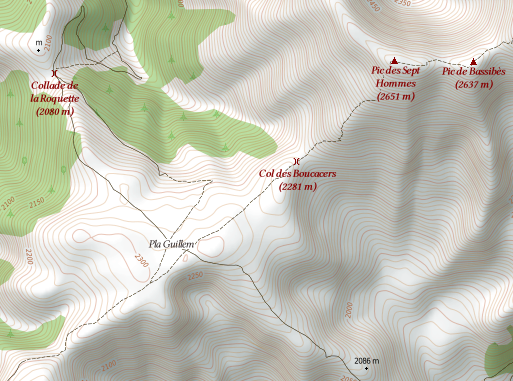
\includegraphics[height=4cm]{../figures/isohypses.png}
%		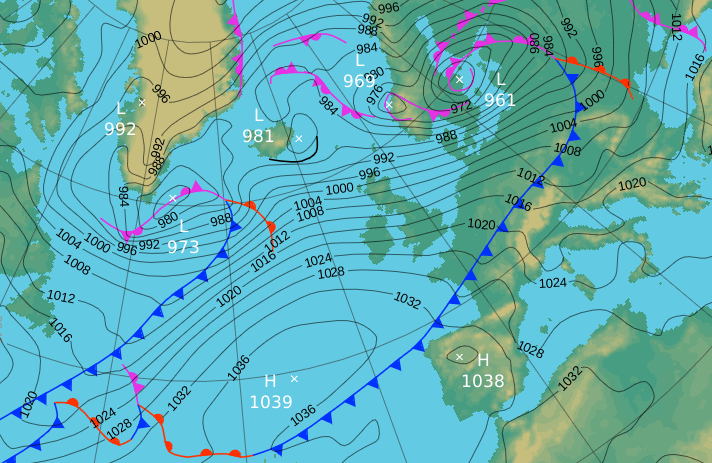
\includegraphics[height=4cm]{../figures/isobar.png}
%	\end{tabular}
%\end{center}
%\end{exemple}
%
%
%Pour les fonctions de $\R^3$ dans $\R$, les ensembles de niveau sont appelés \emph{surfaces de niveau}. Ces surfaces sont des sous-ensembles de $\R^3$ et cela permet de représenter la fonction alors qu'il serait délicat de représenter son graphe, qui est un sous-ensemble de $\R^4$.  


\sld{\vfill\pagebreak[5]}%%%%%%%%%%%%%%%
\begin{exemple}
Lorsque la fonction $f:\R^3 \to \R$ est polynomiale, on parle de surfaces algébriques. En voici deux exemples classiques :
	\begin{center}
%\tikzexternalenable
		\begin{tabular}{p{.45\textwidth}c}
\tikzsetnextfilename{cours-sphere}
\begin{tikzpicture}
    \begin{axis}[%
	width=.45\textwidth,
        axis equal,
        %width=10cm,
        %height=10cm,
        %axis lines = center,
        xlabel = {$x$},
        ylabel = {$y$},
        zlabel = {$z$},
        zlabel style={rotate=-90},
	%ticks=none,
        %enlargelimits=0.3,
        %view/h=45,
        %scale uniformly strategy=units only,
    ]
    \addplot3[ surf, opacity = 0.5, samples=21, domain=-1:1,y domain=0:2*pi, z buffer=sort] ({sqrt(1-x^2) * cos(deg(y))}, {sqrt( 1-x^2 ) * sin(deg(y))},
     x);
    \addplot3[ surf, opacity = 0.5, samples=21, domain=-1:1,y domain=-pi/4:2*pi-pi/2, z buffer=sort] ({sqrt(4-x^2) * cos(deg(y))}, {sqrt(4-x^2 ) * sin(deg(y))},
     x);
    \end{axis}

\end{tikzpicture}&
\tikzsetnextfilename{hyperbol}
\begin{tikzpicture}
    \begin{axis}[width=.45\textwidth,
        axis equal,
            xmin=-2,xmax=2,
            ymin=-2,ymax=2,
            zmin=-2,zmax=2,
            xlabel={$x$},
            ylabel={$y$},
            zlabel={$z$},
            zlabel style={rotate=-90},
            %view={60}{40}
    ]
        % x^2+y^2-z^2=1
        \addplot3[surf,opacity=.5,domain=1:2,y domain=0:2*pi,samples=15]({x*cos(deg(y))},{x*sin(deg(y))},{sqrt(x^2-1)});    
        \addplot3[surf,opacity=.5,domain=1:2,y domain=0:2*pi,samples=15]({x*cos(deg(y))},{x*sin(deg(y))},{-sqrt(x^2-1)});    

        % x^2+y^2-z^2=2
        %\addplot3[mesh,opacity=.5,domain=1:2,y domain=0:2*pi,samples=60,z buffer=sort]({x*cos(deg(y))},{x*sin(deg(y))},{(x*x-2)^.5 });    
        %\addplot3[mesh,opacity=.5,domain=1:2,y domain=0:2*pi,samples=60]({x*cos(deg(y))},{x*sin(deg(y))},{-(x*x-2)^.5 });    
    \end{axis}
\end{tikzpicture}\\												
			Sphère : surfaces de niveau $1$ et $4$ (tronquée) de la fonction $f(x,y,z) = x^2 + y^2 + z^2 $&
			Paraboloïde : la surface de niveau $1$ de  $f(x,y,z) = x^2 + y^2 - z^2$
		\end{tabular}
%\tikzexternaldisable
	\end{center}
	\pl{Bien d'autres exemples a cette adresse :  \url{{http://www.mathcurve.com/surfaces/algebricsu/algebricsu.shtml}} \fbox{\qrcode[,height=.5cm]{http://www.mathcurve.com/surfaces/algebricsu/algebricsu.shtml}}}
\end{exemple}


\sld{\vfill\pagebreak[5]}%%%%%%%%%%%%%%%
\subsection{Les fonctions partielles}
\begin{definition}
	\'Etant donné une fonction $f:\R^2 \to \R$ définie sur tout le plan et un nombre $a\in\R$, les fonctions partielles de $f$ sont $f^1_a,f^2_a : \R\to\R$ définies pour tout $t\in\R$ par :
	\[
		f^1_a(t) = f(a,t) \quad \text{ et } \quad f^2_a(t) = f(t,a).
	\]
\end{definition}

%Dans le cas $n=2$ il y a deux fonctions partielles : si $f:\R^2 \to \R$ et $a\in\D(f)$ alors $f^1_a(\cdot) = f(a,\cdot)$ et $f^2_a (\cdot) = f(\cdot,a)$.
Le graphe des fonctions partielles peut être déduit du graphe $\mathcal G_f$ de $f$ en prenant l'intersection entre $\mathcal G_f$ et les plans (verticaux) d'équation $x=a$ et $y=a$, respectivement.

%\tikzexternalenable
\begin{tabular}{cc}
	\tikzsetnextfilename{cours-partial}
	\begin{tikzpicture}[scale=.7]
		\def\cut{6}
		\def\formgnuplot{sin(sqrt(x**2 + y**2)) /sqrt(x**2 + y**2)};
		\def\form{sin(deg( (x^2 + (\cut) ^2)^.5)) /(x^2 + (\cut) ^2)^.5};
		\begin{axis}[
			xlabel = {$x$},
        ylabel = {$y$},
        zlabel = {$z$},
        zlabel style={rotate=-90},
			xmin=-10,xmax=10,ymin=-10,ymax=10,zmin=-.3,zmax=1.3]
			\addplot3[surf,y domain=-10:10,domain=-10:\cut, samples=40,samples y= 50,colormap/cool,opacity=.8,id=zozo2]gnuplot {\formgnuplot};
			\draw[opacity=.5,fill=red!50,red] (axis cs: \cut,-10,-.3)-- (axis cs: \cut,10,-0.3) -- (axis cs: \cut,10,1.3) -- (axis cs: \cut,-10,1.3) -- cycle ;
			\addplot3[domain=-10:10,samples=50,samples y=0,red,ultra thick] (\cut,x,\form);
			\addplot3[surf,y domain=-10:10, domain = \cut:10,samples=10,samples y= 50,colormap/cool,opacity=.8,id=zozo]gnuplot {\formgnuplot};
		\end{axis}
	\end{tikzpicture}	                & 

	\tikzsetnextfilename{cours-partial2}
	\begin{tikzpicture}[scale=.7]
		\begin{axis}[
		xlabel = {$y$},
        ylabel = {$z$},
        ylabel style={rotate=-90},
			xmin=-10,xmax=10,ymin=-.3,ymax=1.3]
			\def\cut{6};
			%	\def\formgnuplot{sin(sqrt(x**2 + y**2)) /sqrt(x**2 + y**2)};
			\def\form{sin(deg( (x^2 + (\cut) ^2)^.5)) /(x^2 + (\cut) ^2)^.5};
			\addplot[domain=-10:10,samples=60,blue,ultra thick] {\form};
		\end{axis}
	\end{tikzpicture} \\
	Graphe de $f(x,y) = \sin(\sqrt{x^2 + y^2}) /\sqrt{x^2 + y^2}$ & Graphe de $f^1_a:y \mapsto f(a,y)$ où $a = 6$
\end{tabular}

%\tikzexternaldisable

%\tikzexternalenable
\begin{tabular}{cc}
\tikzsetnextfilename{cours-partial3}
			\begin{tikzpicture}[scale=.7]
				\def\cut{-2};
				\begin{axis}[
					xlabel = {$x$},
        ylabel = {$y$},
        zlabel = {$z$},
        zlabel style={rotate=-90},
					xmin=-10,xmax=10,ymin=-10,ymax=10,zmin=-.3,zmax=1.3]
					\addplot3[surf,domain=-10:10,y domain=\cut:10, samples=50,samples y= 30,colormap/cool,opacity=.8,id=zozo]gnuplot {sin(sqrt(x**2 + y**2)) / sqrt(x**2 + y**2)};
					\draw[opacity=.5,fill=red!50,red] (axis cs: -10,\cut,-.3)-- (axis cs: 10,\cut,-0.3) -- (axis cs: 10,\cut,1.3) -- (axis cs: -10,\cut,1.3) -- cycle ;
					\addplot3[domain=-10:10,samples=50,samples y=0,red,ultra thick] (x,\cut,{sin(deg( (x^2 + (\cut) ^2)^.5)) /(x^2 + (\cut)^2)^.5});
					\addplot3[surf,domain=-10:10, y domain = -10:\cut,samples=50,samples y= 20,colormap/cool,opacity=.8,id=zozo]gnuplot {sin(sqrt(x**2 + y**2)) / sqrt(x**2 + y**2)};
				\end{axis}
			\end{tikzpicture}	                &
\tikzsetnextfilename{cours-partial4}
			\begin{tikzpicture}[scale=.7]
				\begin{axis}[
				xlabel = {$x$},
        ylabel = {$z$},
        ylabel style={rotate=-90},
					xmin=-10,xmax=10,ymin=-.3,ymax=1.3]
				\def\cut{-2};
			%	\def\formgnuplot{sin(sqrt(x**2 + y**2)) /sqrt(x**2 + y**2)};
				\def\form{sin(deg( (x^2 + (\cut) ^2)^.5)) /(x^2 + (\cut) ^2)^.5};
				\addplot[domain=-10:10,samples=60,blue,ultra thick] {\form};
				\end{axis}
			\end{tikzpicture}	                
 \\
	Graphe de $f(x,y) = \sin(\sqrt{x^2 + y^2}) /\sqrt{x^2 + y^2}$ & Graphe de $f^2_b:x\mapsto f(x,b)$ où $b = -2$
\end{tabular}

%\tikzexternaldisable

\sld{\vfill\pagebreak[5]}%%%%%%%%%%%%%%%
\section[Fonctions de plusieurs variables à valeurs vectorielles]{Représentation des fonctions de plusieurs variables à valeurs vectorielles}

\subsection{Définition}

\begin{definition}
	Une fonction $f$ de plusieurs variables à valeurs vectorielles (aussi appelée \emph{champ de vecteurs}) est une fonction définie sur une partie $\D$ de $\R^n$ ($n\geq 1$) et à valeurs dans $\R^m$ ($m\geq 1$). Dans ce cas, il existe $m$ fonctions $f_1,\cdots,f_m : \R^n \to \R$ telles que pour tout $x =(x_1,x_2,\cdots,x_n)\in \R^n$ de $\D$ on ait $f(x) = (f_1(x),\cdots,f_m(x)) \in \R^m$.
\end{definition}

\sld{\vfill\pagebreak[5]}%%%%%%%%%%%%%%%
\subsection{Représentation des champs de vecteurs}

Lorsque $m=n=2$ ou $3$, on peut représenter l'application $\R^n \to \R^n$ par une collection de flèches~: en chaque point $x\in\R^n$ est représenté un vecteur $f(x)\in \R^n$. La terminologie ``champ de vecteurs'' est donc appropriée.

\sld{\vfill\pagebreak[5]}%%%%%%%%%%%%%%%
\begin{exemple}
	Le champ de vecteurs $f(x,y) = \frac{0.15}{\sqrt{1+(x-y)^2}} \left(1, x-y\right )$ défini sur $\D = \R^2$ :
	\begin{center}
		%\tikzexternalenable
			\tikzsetnextfilename{cours-vf2d}	
		\def\length{sqrt(1+(x-y)^2)}
\begin{tikzpicture}
\begin{axis}[domain=-3:3, view={0}{90},xlabel = $x$,ylabel=$y$,ylabel style={rotate=-90},]
\addplot3[blue, quiver={u={1/(\length)}, v={(x-y)/(\length)}, scale arrows=0.15}, -stealth,samples=20] {0};
\end{axis}
\end{tikzpicture}

		\tikzexternaldisable
	\end{center}
\end{exemple}

\sld{\vfill\pagebreak[5]}%%%%%%%%%%%%%%%
\begin{exemple}
	Un champ de vecteurs $f:\R^3 \to \R^3$ défini sur $\D =\left\{ x^2 + y^2 + z^2 =1 \right\}$. On a $f(x,y,z) = \begin{psmallmatrix}f_1(x,y,z)\\ f_2(x,y,z) \\ f_3(x,y,z)\end{psmallmatrix} \in \R^3$. En chaque point du domaine de définition on a donc un vecteur (``une flèche'') représenté par un champ de vecteurs :
	\begin{center}
		\tikzexternalenable
			\tikzsetnextfilename{cours-vf3d}	
		%% helper macros
%: Styles for XYZ-Coordinate Systems
%: isometric  South West : X , South East : Y , North : Z
\tikzset{isometricXYZ/.style={x={(-0.866cm,-0.5cm)}, y={(0.866cm,-0.5cm)}, z={(0cm,1cm)}}}

%: isometric South West : Z , South East : X , North : Y
\tikzset{isometricZXY/.style={x={(0.866cm,-0.5cm)}, y={(0cm,1cm)}, z={(-0.866cm,-0.5cm)}}}

%: isometric South West : Y , South East : Z , North : X
\tikzset{isometricYZX/.style={x={(0cm,1cm)}, y={(-0.866cm,-0.5cm)}, z={(0.866cm,-0.5cm)}}}

%% document-wide tikz options and styles
\begin{tikzpicture} [scale=2, isometricZXY, line join=round,
        opacity=.75, text opacity=1.0,%
        %>=latex,
        inner sep=0pt,%
        outer sep=2pt,%
    ]
    \def\h{5}
    \shade[ball color=red!10!white,opacity=0.20] (0,0) circle (1.2cm);
    %Movement arrows
    \foreach \t in {225,235,...,295}
	\foreach \f in {50,40,...,0}
	    \draw [blue, opacity=1.0, ->, thick]
		({sin(\f - \h)*cos(\t - \h)}, {sin(\f - \h)*sin(\t - \h)}, {cos(\f - \h)})
		-- ({(1 + 0.2*cos(90 - \f))*sin(\f - \h)*cos(\t - \h)},
		    {(1 + 0.2*cos(90 - \f))*sin(\f - \h)*sin(\t - \h)},
		    {(1 + 0.2*cos(90 - \f))*cos(\f - \h)});

    \foreach \t in {125,135,...,205}
	\foreach \f in {110,100,...,0}
	    \draw [blue, <-, thick]
		({(1 + 0.2*cos(90 - \f))*sin(\f - \h)*cos(\t - \h)},
		 {(1 + 0.2*cos(90 - \f))*sin(\f - \h)*sin(\t - \h)},
		 {(1 + 0.2*cos(90 - \f))*cos(\f - \h)})
		-- ({sin(\f - \h)*cos(\t - \h)},{sin(\f - \h)*sin(\t - \h)},{cos(\f - \h)});
    \foreach \t in {35,45,...,115}
	\foreach \f in {130,120,...,0}
	    \draw [blue, opacity=1.0 ,->, thick]
		({sin(\f - \h)*cos(\t - \h)}, {sin(\f - \h)*sin(\t - \h)}, {cos(\f - \h)})
		-- ({(1 + 0.2*cos(90 - \f))*sin(\f - \h)*cos(\t - \h)},
		    {(1 + 0.2*cos(90 - \f))*sin(\f - \h)*sin(\t - \h)},
		    {(1 + 0.2*cos(90 - \f))*cos(\f - \h)});

    \foreach \t in {-55,-45,...,25}
	\foreach \f in {130,120,...,0}
	    \draw [blue, <-, thick]
		({(1 + 0.2*cos(90 - \f))*sin(\f - \h)*cos(\t - \h)},
		 {(1 + 0.2*cos(90 - \f))*sin(\f - \h)*sin(\t - \h)},
		 {(1 + 0.2*cos(90 - \f))*cos(\f - \h)})
	      -- ({sin(\f - \h)*cos(\t - \h)},{sin(\f - \h)*sin(\t - \h)},{cos(\f - \h)});

\end{tikzpicture}

		%\tikzexternaldisable

	\end{center}
\end{exemple}

%\section{Les courbes du plan et de l'espace}

